\subsubsection{Unit testing}
Complementing our set of behavioural tests are unit tests primarily focusing on TaxEngine's taxAmount calculation. 'taxAmount' was refactored to delegate the taxing of specific tax groups to disparate public helper methods. By creating tests that target both the encompassing taxAmount() as well as the other more specific (taxBasedOnMaritalStatus, taxBasedOnChildren, taxBasedOnEducationStatus), the test environment was able to zoom in on where the defects occurred more quickly. A failure in unit test targeting taxAmount's  tax calculation, would be accompanied by another failure that on one of the helper methods. Thus we were able to quickly locate the defect sources. 

\par
Similar to the behavioural tests, there were far too many combinations of tax code inputs and salaries to consider creating individual test cases for each. The better solution was to use JUnit's @ParameterizedTest annotation which allows a single test to be executed multiple times with different input arguments that can be provided through a method returning a Stream of Arguments (\javainline{Stream<Arguments>}). 

\begin{figure}[H]
\centering
\begin{mdframed}
\centering
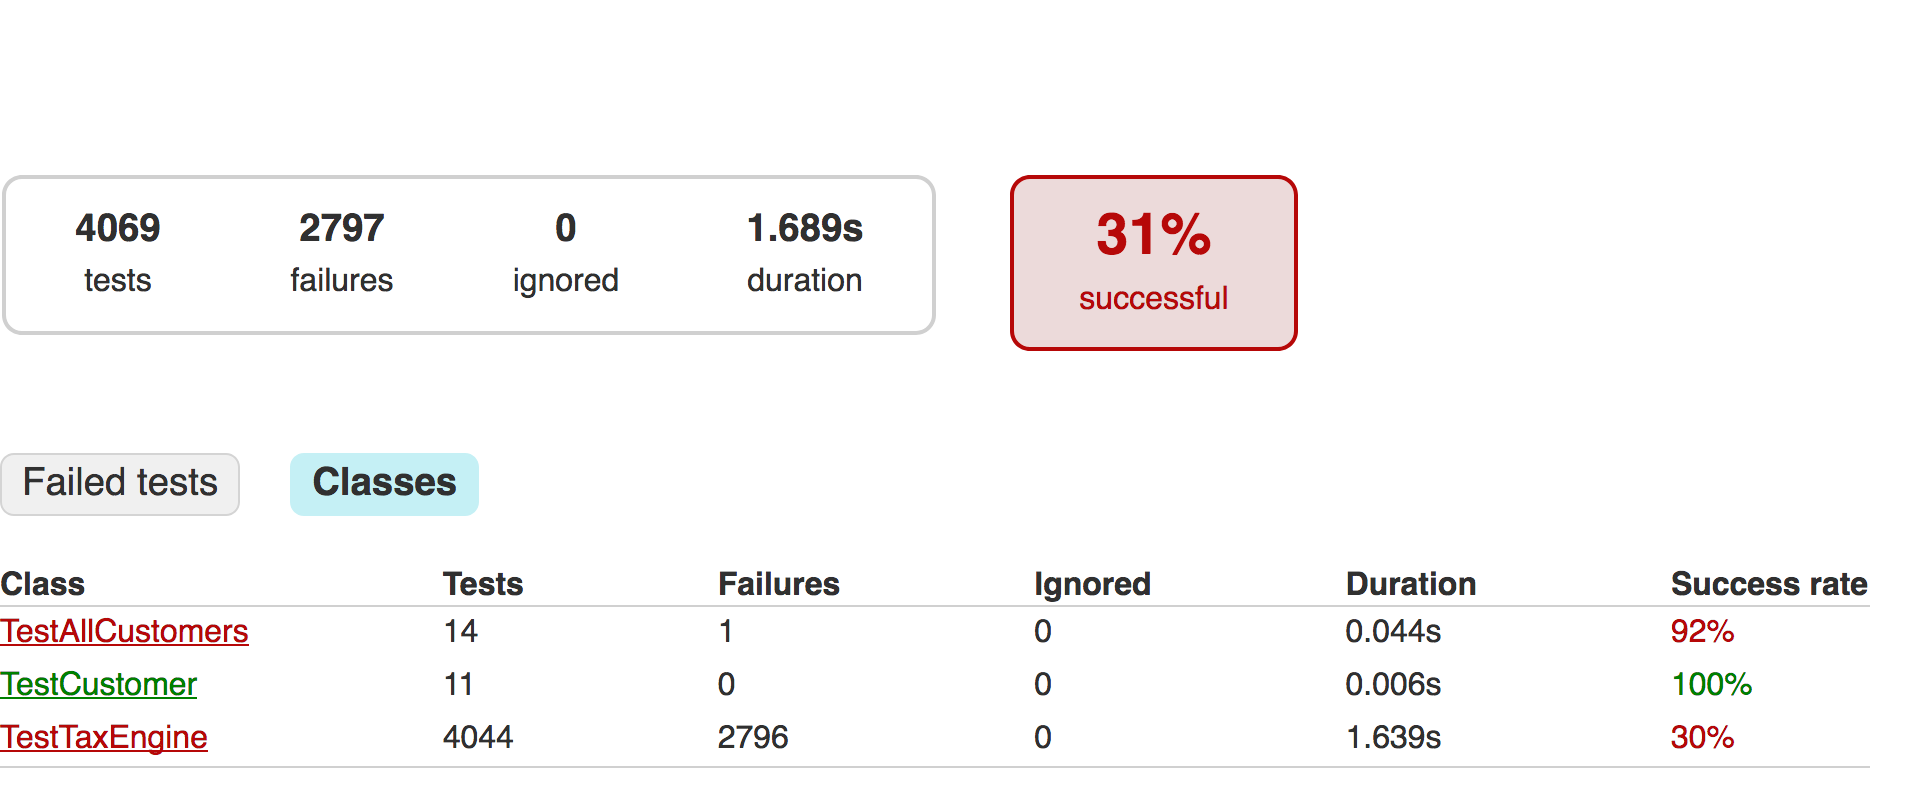
\includegraphics[scale=0.5]{res/unit-test.png}
\caption{JUnit Test Report}    
\end{mdframed}
\end{figure}